\section{BLOCK DIAGRAMS}
\subsection{System Architecture}
\begin{figure}[h]
    \centering
    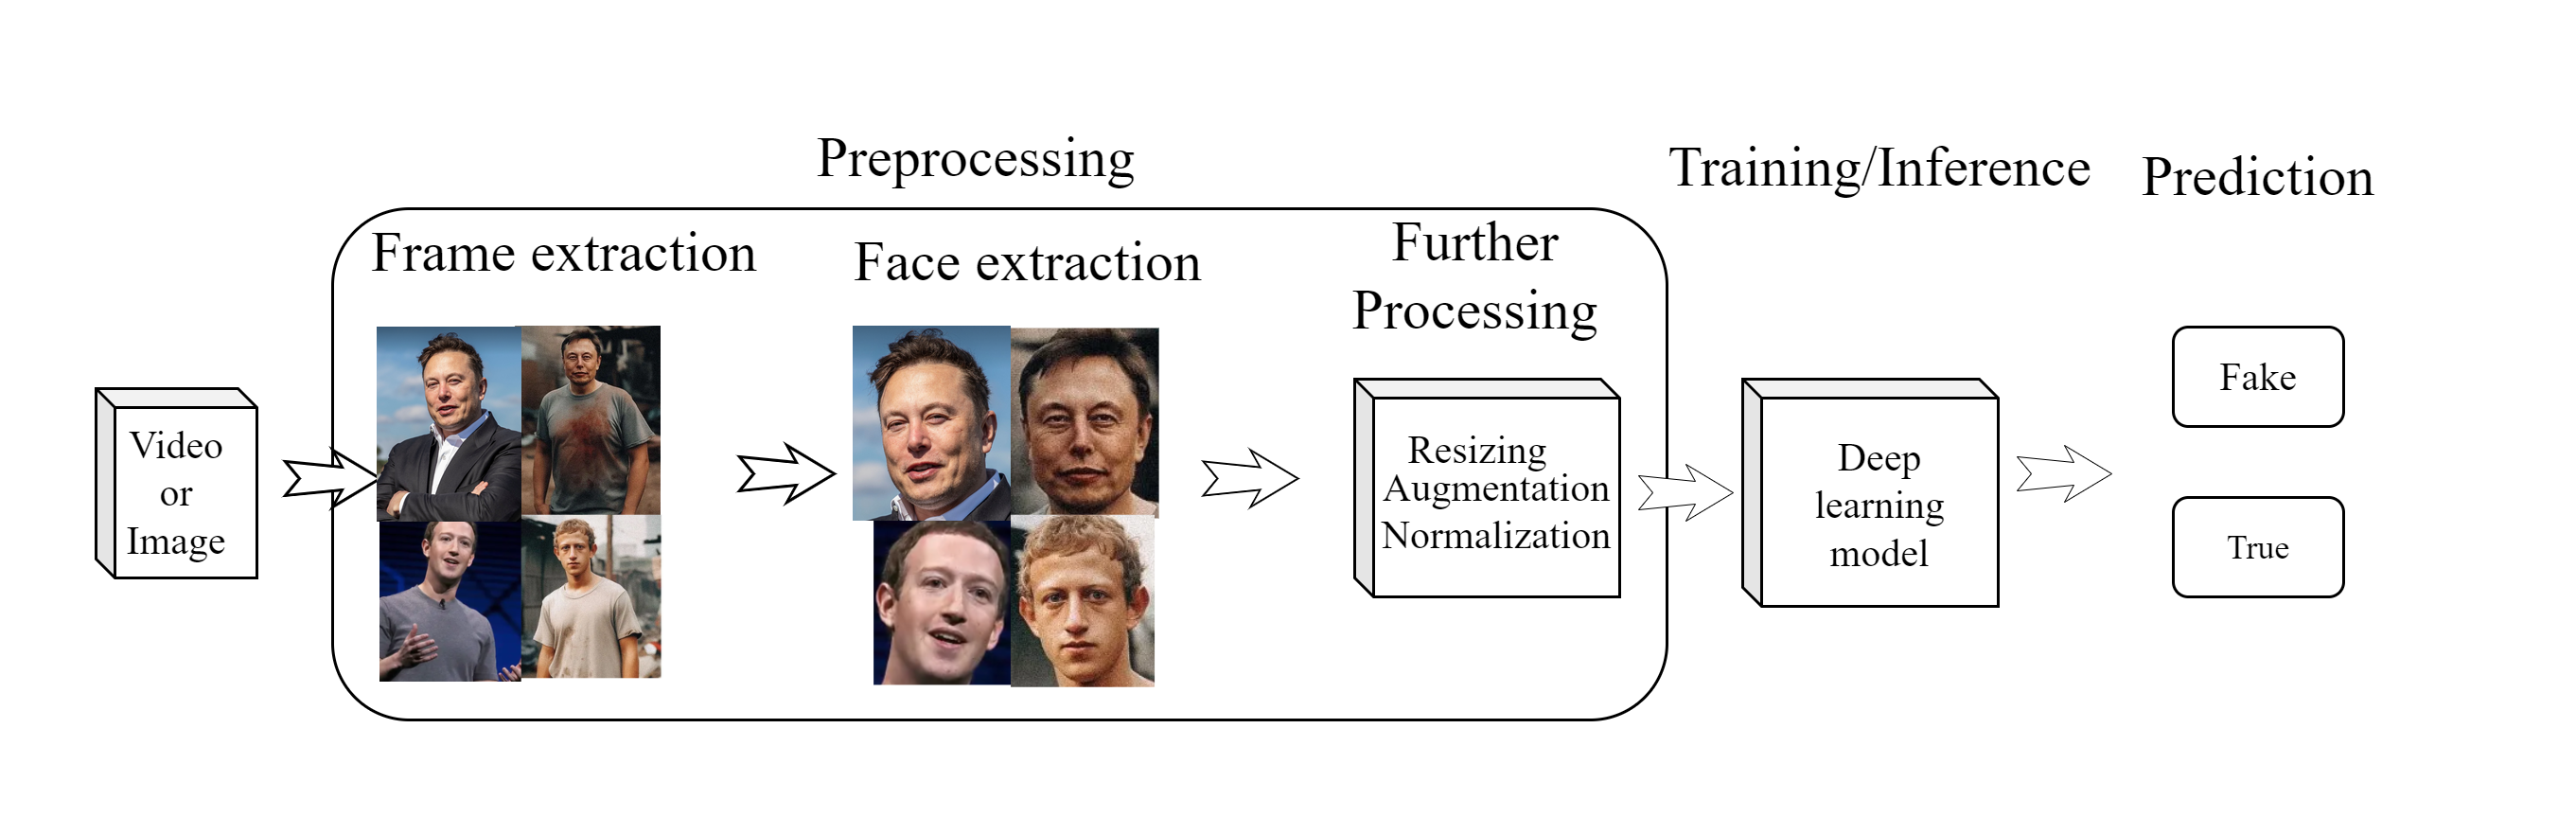
\includegraphics[width= 6.5in ]{img/systemachitecture.drawio.png}
    \caption{System Architecture}

\end{figure}
\justify
The system architecture of our project involves multiple steps. Initially, frames are extracted from the input video or obtained directly from an image. These frames then undergo face extraction, where faces are identified and cropped using face detection algorithms. The extracted faces are resized to a standardized size and undergo normalization to ensure consistent pixel values. The preprocessed face images are then fed into a deep learning model for classification. The model analyzes the features and patterns in the images to determine whether they are real or fake. Finally, the system produces the output, indicating the authenticity of the input video or image as either real or fake.
